\section{Equations of motion}
\begin{frame}{Configuration vector}
  \[  
  \vec{q} =
  \begin{bmatrix}
    \theta_{1} & \theta_{2} & \theta_{3} & q_{x} & q_{y} & q_{z}
  \end{bmatrix} \transpose
  \]
  \vskip-0.1in
  \begin{columns}
    \begin{column}{0.55\textwidth}
      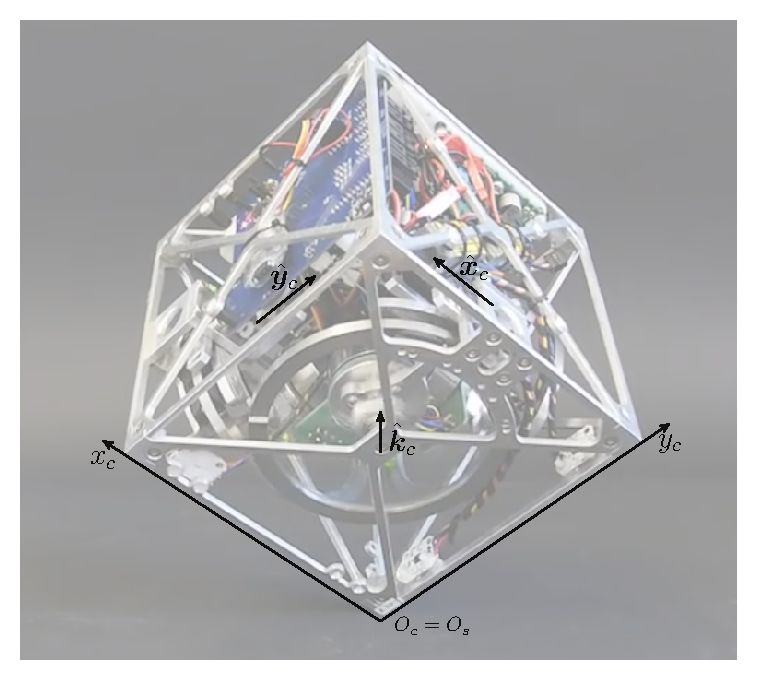
\includegraphics[width=\columnwidth]{cubli}
    \end{column}
    \begin{column}{0.6\textwidth}
      \begin{block}{Attitude}
        \begin{itemize}
        \item[-] Body fixed reference frame $\{C\} = (O_c; \hat{\vec{i}}_c, \hat{\vec{j}}_c, \hat{\vec{k}}_c)$
        \item[-] Inertial reference frame $\{S\} = (O_s; \hat{\vec{i}}_s, \hat{\vec{j}}_s, \hat{\vec{k}}_s)$
        \item[-] $R_{SC}(\vec{\theta}) = R_z(\theta_1)R_y(\theta_2)R_x(\theta_3)$
        \end{itemize}
      \end{block}
      \begin{block}{Flywheels}
        $q_x$, $q_y$ and $q_z$ are the flywheel angular positions
      \end{block}
    \end{column}
  \end{columns}
\end{frame}

\begin{frame}{Notation \footnote[frame]{All quantities expressed in $\{C\}$}}
  \begin{columns}[t]
    \begin{column}{0.5\textwidth}
      \begin{block}{Velocities}
        \begin{itemize}
        \item[-] $\prescript{c}{}{\vec{v}}_{G_{c}}$: cubic frame CoM linear velocity
        \item[-] $\prescript{c}{}{\vec{v}}_{G_{i}}$: i-th flywheel CoM linear velocity
        \item[-] $\prescript{c}{}{\vec{\omega}}_{c}$: cubic frame angular velocity
        \item[-] $\prescript{c}{}{\vec{\omega}}_{i}$: i-th flywheel angular velocity
        \end{itemize}
      \end{block}
    \end{column}
    \begin{column}{0.5\textwidth}
      \begin{block}{Inertial quantities}
        \begin{itemize}
        \item[-] $m_c$: cubic frame mass
        \item[-] $m_i$: i-th flywheels mass
        \item[-] $\prescript{c}{}{\mathfrak{J}}_{G_{c}}$: cubic frame inertia matrix of the 
        \item[-] $\prescript{c}{}{\mathfrak{J}}_{G_{i}}$: i-th flywheel inertia matrix
        \end{itemize}
      \end{block}
    \end{column}
  \end{columns}
\end{frame}

\begin{frame}{Inertia matrices and parameters}
  \begin{columns}
    \begin{column}{0.55\textwidth}
      \begin{block}{Inertia matrices}
        \vskip-0.1in
      \[
  \begin{split}
    &\prescript{c}{}{\mathfrak{J}}_{G_{x}} = 
    \left[
      \begin{smallmatrix}
        \frac{m r^2}{2} & 0 & 0\\
      0 & \frac{m\left(h^2 + 3 r^2 \right)}{12}  & 0\\
      0 & 0 & \frac{m\left(h^2 + 3 r^2 \right)}{12}
      \end{smallmatrix}
      \right]\\
    &\prescript{c}{}{\mathfrak{J}}_{G_{y}} = 
    \left[
    \begin{smallmatrix}
      \frac{m\left(h^2 + 3 r^2 \right)}{12} & 0 & 0\\
      0 & \frac{m r^2}{2} & 0\\
      0 & 0 & \frac{m\left(h^2 + 3 r^2 \right)}{12}
    \end{smallmatrix}
    \right] \\
    &\prescript{c}{}{\mathfrak{J}}_{G_{z}} = 
    \left[
      \begin{smallmatrix}
        \frac{m\left(h^2 + 3 r^2 \right)}{12} & 0 & 0\\
        0 & \frac{m\left(h^2 + 3 r^2 \right)}{12} & 0\\
      0 & 0 & \frac{m r^2}{2}
      \end{smallmatrix}
      \right]
    \\
    &\prescript{c}{}{\mathfrak{J}}_{G_{c}} = 
    \left[
      \begin{smallmatrix}
      \frac{m_c a^2}{6} & 0 & 0\\
      0 & \frac{m_c a^2}{6} & 0\\
      0 & 0 & \frac{m_c a^2}{6}
    \end{smallmatrix}
    \right]
  \end{split}
  \] 
  \end{block}
  \end{column}
    \begin{column}{0.5\textwidth}
      \begin{block}{Parameters}
        \begin{itemize}
        \item[-] $M = \SI{2.5}{kg}$ (cubic frame mass)
        \item[-] $a = \SI{0.15}{m}$ (cube side)
        \item[-] $m = \SI{0.204}{kg}$ (flywheel mass)
        \item[-] $r = \SI{0.05}{m}$ (flywheel radius)
        \item[-] $h = \SI{0.005}{m}$ (flywheel height)
        \end{itemize}
      \end{block}
    \end{column}
  \end{columns}
\end{frame}

\begin{frame}[shrink=15]{Kinematics}
  \begin{columns}
    \begin{column}{0.5\textwidth}
      \[
      \begin{split}
        & \prescript{c}{}{\vec{\omega}}_c = 
        \begin{bmatrix}
          \prescript{c}{}{J}_{\omega} (\vec{\theta}) & 0_{3 \times 3}
        \end{bmatrix}\vec{\dot{q}} 
        = \prescript{c}{}{J}_{\omega} (\vec{q}) \vec{\dot{q}}\\
        & \prescript{c}{}{\vec{\omega}}_x = 
        \begin{bmatrix}
          \prescript{c}{}{\tilde{J}_{\omega}} & \vec{e}_1 & \vec{0} & \vec{0}
        \end{bmatrix} \dot{\vec{q}} = \prescript{c}{}{J}_{\omega_{x}} \dot{\vec{q}}\\
        &  \prescript{c}{}{\vec{\omega}}_y = 
        \begin{bmatrix}
          \prescript{c}{}{\tilde{J}_{\omega}} & \vec{0} & \vec{e}_2 & \vec{0}
        \end{bmatrix} \dot{\vec{q}} = \prescript{c}{}{J}_{\omega_{y}} \dot{\vec{q}}\\
        &  \prescript{c}{}{\vec{\omega}}_z = 
        \begin{bmatrix}
          \prescript{c}{}{\tilde{J}_{\omega}} & \vec{0} & \vec{0} & \vec{e}_3
        \end{bmatrix} \dot{\vec{q}} = \prescript{c}{}{J}_{\omega_{z}} \dot{\vec{q}}
      \end{split}
      \]
    \end{column}
    \begin{column}{0.5\textwidth}
      \[
      \prescript{c}{}{\tilde{J}}_{\omega} (\vec{q}) =
      \begin{bmatrix}
        -s_2 & 0 & 1 \\
        c_2 s_3 & c_3  & 0\\
        c_2 c_3 & -s_3 & 0
      \end{bmatrix}
      \]
    \end{column}
  \end{columns}
  \[
  \prescript{c}{}{\vec{v}}_{\vec{G}_{i}} =
  \cancelto{0}{\prescript{c}{}{\vec{v}}_{O_{c}}}_{\footnote[frame]{Spherical joint in $O_c = O_s$}} + \prescript{c}{}{\unitvec{\omega}}_c \prescript{c}{}{\vec{G}}_*
  = -\prescript{c}{}{\unitvec{G}}_* \prescript{c}{}{\vec{\omega}}_c
  = -\prescript{c}{}{\unitvec{G}}_* \prescript{c}{}{J_{\omega}} \dot{\vec{\theta}}
  = -\prescript{c}{}{\unitvec{G}}_* \prescript{c}{}{\tilde{J}_{\omega}} \dot{\vec{q}}
  \]
  \[
  \prescript{c}{}{\vec{G}}_{c} = 
  \begin{bmatrix}
    a/2 \\
    a/2 \\
    a/2
  \end{bmatrix} \quad
  \prescript{c}{}{\vec{G}}_x = 
  \begin{bmatrix}
    0 \\
    a/2 \\
    a/2
  \end{bmatrix} \quad
  \prescript{c}{}{\vec{G}}_y = 
  \begin{bmatrix}
    a/2 \\
    0 \\
    a/2
  \end{bmatrix} \quad
  \prescript{c}{}{\vec{G}}_z = 
  \begin{bmatrix}
    a/2 \\
    a/2 \\
    0
  \end{bmatrix}
  \]
\end{frame}

\begin{frame}[shrink=30]{Equation in standard manipulator form}
  \[
  B(\vec{q}) \ddot{\vec{q}} + C(\vec{q}, \dot{\vec{q}}) \dot{\vec{q}} + \vec{G}(\vec{q}) = \vec{Q}
  \]
  \begin{block}{Joint space inertia matrix $B(\vec{q})$}
    \[
    \begin{split}
      B(\vec{q}) &= \cubicFrame{m_c \prescript{c}{}{J}_{\omega}\transpose \prescript{c}{}{\unitvec{G}}_{c} \transpose  \prescript{c}{}{\unitvec{G}}_{c} \prescript{c}{}{J}_{\omega}} + \cubicFrame{\prescript{c}{}{J}_{\omega}\transpose  \prescript{c}{}{\mathfrak{J}}_{G_{c}} \prescript{c}{}{J}_{\omega}} + 
      \qx{m_x \prescript{c}{}{J}_{\omega}\transpose \prescript{c}{}{\unitvec{G}}_{x} \transpose  \prescript{c}{}{\unitvec{G}}_{x} \prescript{c}{}{J}_{\omega}} + 
      \qx{\prescript{c}{}{J}_{\omega_{x}}\transpose  \prescript{c}{}{\mathfrak{J}}_{G_{x}} \prescript{c}{}{J}_{\omega_{x}}} \\
      &+ \qy{m_y \prescript{c}{}{J}_{\omega}\transpose \prescript{c}{}{\unitvec{G}}_{y} \transpose  \prescript{c}{}{\unitvec{G}}_{y} \prescript{c}{}{J}_{\omega}} + 
      \qy{\prescript{c}{}{J}_{\omega_{y}}\transpose  \prescript{c}{}{\mathfrak{J}}_{G_{y}} \prescript{c}{}{J}_{\omega_{y}}} 
      + \qz{m_z \prescript{c}{}{J}_{\omega}\transpose \prescript{c}{}{\unitvec{G}}_{z} \transpose  \prescript{c}{}{\unitvec{G}}_{z} \prescript{c}{}{J}_{\omega}} + \qz{\prescript{c}{}{J}_{\omega_{z}}\transpose  \prescript{c}{}{\mathfrak{J}}_{G_{z}} \prescript{c}{}{J}_{\omega_{z}}}\\
      & = B(\theta_2, \theta_3)
    \end{split}
    \]
  \end{block}
  \begin{columns}
    \begin{column}{0.5\textwidth}
      \begin{block}{Coriolis $C(\vec{q}, \dot{\vec{q}})$}
        \[
        C_{ij} = \sum_{k=1}^6{\Gamma^i_{jk} \dot{q}_k}
        \]
        \[
        \Gamma^i_{jk} = \frac{1}{2} \left ( \frac{\partial B_{ij}}{\partial q_k}
        + \frac{\partial B_{ik}}{\partial q_j}
        - \frac{\partial B_{jk}}{\partial q_i}\right)
        \]
      \end{block}
    \end{column}
    \begin{column}{0.5\textwidth}
      \begin{block}{Gravitational forces $G(\vec{q})$}
        \[
        \vec{G} =\left(\frac{\partial U}{\partial \vec{q}}\right) \transpose
        \]
        \[
        \begin{split}
          U(\vec{q}) = - \prescript{c}{}{\vec{g}} \transpose
          &(\cubicFrame{m_c  \prescript{c}{}{\vec{G}}_c} +
          \qx{m_x  \prescript{c}{}{\vec{G}}_x} \\
          &+\qy{m_y  \prescript{c}{}{\vec{G}}_y} +
          \qz{m_z  \prescript{c}{}{\vec{G}}_z})
        \end{split}
        \]
        \[
        \prescript{c}{}{\vec{g}} = R_{SC}\transpose \prescript{s}{}{\vec{g}} = R_{SC}\transpose 
        \begin{bmatrix}
          0 & 0 & -g
        \end{bmatrix} \transpose
        \]
      \end{block}
    \end{column}
  \end{columns}
\end{frame}

\begin{frame}{Derivation of the generalized forces $\vec{Q}$}
  $\vec{\tau} = \begin{bmatrix}
    \tau_x & \tau_y &\tau_z
  \end{bmatrix} \transpose$ are the torques applied to the flywheels
  \[
  \begin{split}
    Q_i = & \tau_{x} \hat{\vec{i}}_c^{T} \frac{\partial (\prescript{c}{}{\vec{\omega}_x})}{\partial \dot{q}_i} +
    \tau_{y} \hat{\vec{j}}_c^{T} \frac{\partial (\prescript{c}{}{\vec{\omega}_y})}{\partial \dot{q}_i} +
    \tau_{z} \hat{\vec{k}}_c^{T} \frac{\partial (\prescript{c}{}{\vec{\omega}_z})}{\partial \dot{q}_i} -\\
    &\tau_{x} \hat{\vec{i}}_c^{T} \frac{\partial (\prescript{c}{}{\vec{\omega}_c})}{\partial \dot{q}_i} -
    \tau_{y} \hat{\vec{j}}_c^{T} \frac{\partial (\prescript{c}{}{\vec{\omega}_c})}{\partial \dot{q}_i} -
    \tau_{z} \hat{\vec{k}}_c^{T} \frac{\partial (\prescript{c}{}{\vec{\omega}_c})}{\partial \dot{q}_i}
  \end{split}
  \]
  \[
  \vec{Q} =
  \begin{bmatrix}
    0 \\ 0 \\ 0 \\ \vec{\tau}
  \end{bmatrix}
  = F \vec{\tau} = 
  \begin{bmatrix}
    0_{3\times3} \\
    I_{3\times3}
  \end{bmatrix} \vec{\tau}
  \]
  \[ 
  \text{rank}(F) = 3 < 6 \quad \forall \vec{q} \implies \text{underactuated system}
  \]
\end{frame}

\begin{frame}{Equations in control affine form}
  \[
  \begin{split}
    \dot{\tilde{\vec{x}}} &= 
    \begin{bmatrix}
      \tilde{\vec{x}}_2 \\
      - B({\tilde{\vec{x}}_1}) ^ {-1} (C(\tilde{\vec{x}}_1, \tilde{\vec{x}}_2) \tilde{\vec{x}}_2 + \vec{G}(\tilde{\vec{x}}_1)) 
    \end{bmatrix} +
    \begin{bmatrix}
      \vec{0} \\
      B({\tilde{\vec{x}}_1}) ^ {-1} \vec{Q}
    \end{bmatrix}\\
    &=\begin{bmatrix}
    \tilde{\vec{x}}_2 \\
    - B^ {-1} (C \tilde{\vec{x}}_2 + \vec{G}) 
    \end{bmatrix} +
    \begin{bmatrix}
      0_{6\times3} \\
      \left(B({\tilde{\vec{x}}_1}) ^ {-1}\right)_{(:, 4:6)}
    \end{bmatrix}\vec{\tau}\\
    &= \tilde{\vec{f}}(\tilde{\vec{x}}) + \tilde{g}(\tilde{\vec{x}}) \vec{\tau}
    = \tilde{\vec{f}}(\tilde{\vec{x}}) + \tilde{g}(\tilde{\vec{x}}) \vec{u}
  \end{split}
  \]
\end{frame}

\begin{frame}{Equations in control affine form (continued)}
  $B$, $C$ and $\vec{G}$ do \alert{not} depend on $q_x$, $q_y$ and $q_z$ and their dynamics can be neglected
  \[
  \vec{x} =
  \begin{bmatrix}
    \theta_1 & \theta_2 & \theta_3 & \dot{\theta}_1 & \dot{\theta}_2 & \dot{\theta}_3 & \dot{q}_x & \dot{q}_y & \dot{q}_z
  \end{bmatrix}\transpose = \begin{bmatrix}
    \vec{\theta} & \vec{\dot{\theta}} & \vec{\dot{q}}_{wheels}
  \end{bmatrix}\transpose
  \]
  \[
  \begin{cases}
    \dot{\vec{x}} = \vec{f}(\vec{x}) + g(\vec{x}) \vec{u} \\
    \vec{y} = \vec{h}(\vec{x}) =
    \begin{bmatrix}
      \theta_1 &
      \theta_2 &
      \theta_3
    \end{bmatrix} \transpose
  \end{cases}
  \]
  \[
  \begin{split}
    \dot{\vec{x}} &= \vec{f}(\vec{x}) + g(\vec{x})\vec{u}\\
    &=\vec{f}(\vec{x}) +
    \begin{bmatrix}
      0_{3\times3} \\
      \left(B(\theta_2,\theta_3) ^ {-1}\right)_{(:, 4:6)}
    \end{bmatrix}\vec{u}\\
  \end{split}
  \]
\end{frame}

\begin{frame}[shrink = 30]{Equlibrium points}
  \begin{center}
    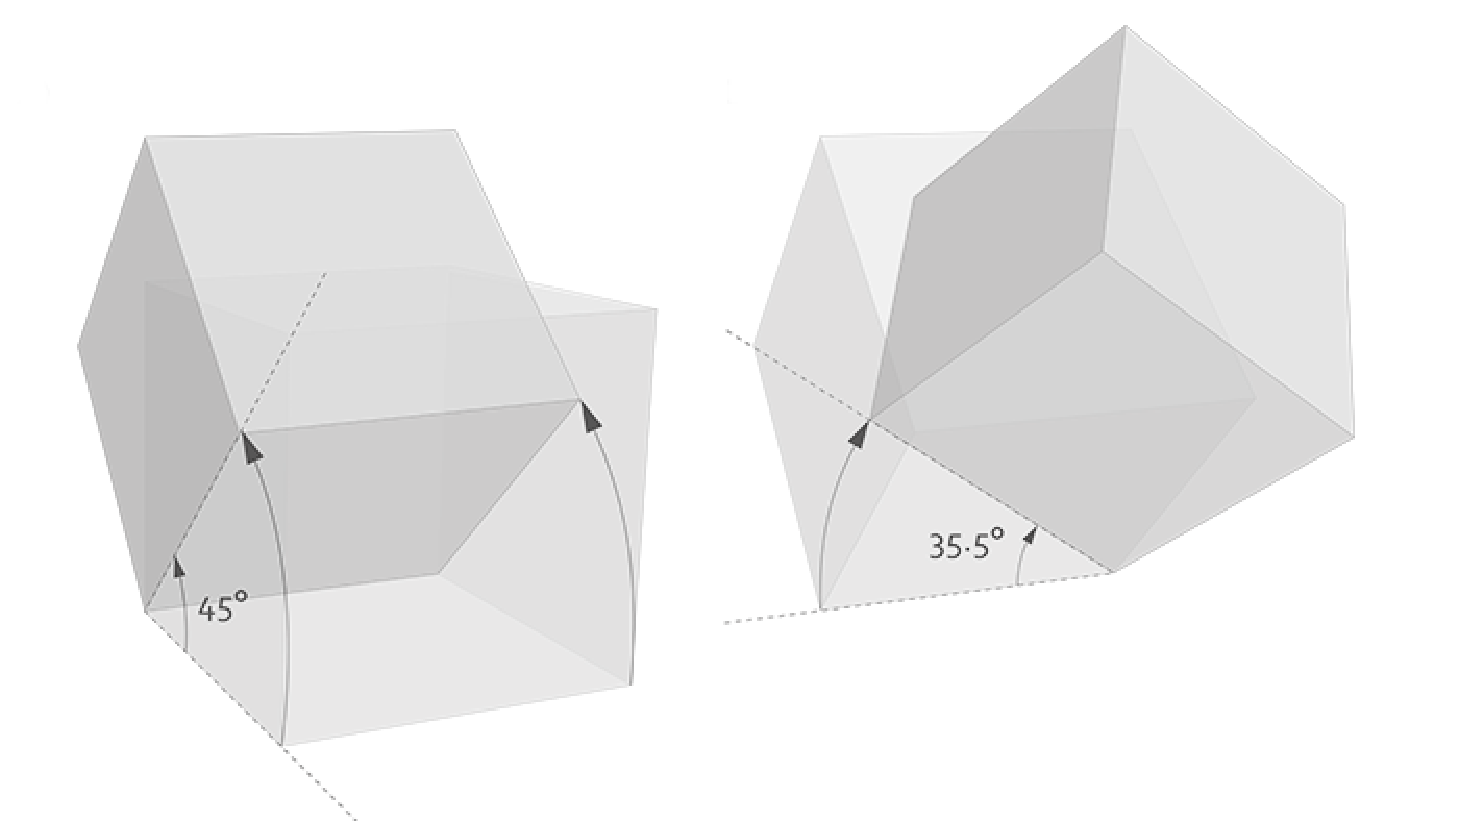
\includegraphics[scale=0.4]{cubli_equilibria}
  \end{center}
  \begin{block}{Upright equilibria (unstable)}
  \[
  \mathcal{E}_{1} = \left\{ \vec{x} \mid \theta_1 \in [-\pi, \pi),\enspace \theta_2 = -\mathrm{atan}\frac{\sqrt{2}}{2},\enspace
   \theta_3 = \frac{\pi}{4},\enspace
    \vec{\dot{\theta}} = \vec{0},\enspace
    \vec{\dot{q}}_{wheels} = \vec{0},\enspace
    \vec{u} = \vec{0}
    \right\}
   \]
  \end{block}
  \begin{block}{Hanging equilibria (stable)}
    \[
    \mathcal{E}_{2} = \left\{
    \vec{x} \mid \theta_1 \in [-\pi, \pi),\enspace
      \theta_2 = \mathrm{atan}\frac{\sqrt{2}}{2},\enspace
    \theta_3 = -\frac{3}{4} \pi,\enspace
    \vec{\dot{\theta}} = \vec{0},\enspace
    \vec{\dot{q}}_{wheels} = \vec{0},\enspace
    \vec{u} = \vec{0}
    \right\}
    \]
  \end{block}
\end{frame}
